\subsection{Preliminary phase}\label{subsec:preliminary-phase}
The preliminary phase still consists of background subtraction and keyboard detection, but the process to follow is much
faster, intuitive and automated.

All the single steps of this phase are shown in~\autoref{fig:preprocessing}.

\paragraph{Image acquisition}
As soon as the application is opened, the user can immediately go to the preliminary step of keyboard detection.
Due to the high mobility of the smartphone and the immediate visual feedback from the screen,
no real background subtraction process is required during this phase: a perimeter is drawn on the smartphone screen
around the area within which the application expects the user to frame the drawn keyboard.

When the user frames the keyboard in the perimeter and presses the button to start the detection process,
the application takes an image with a resolution of $1280 \times 720$, a reasonable resolution for all modern smartphones,
and cuts off from the image all the area outside the perimeter, keeping only the area where the keyboard is located.
This makes the background subtraction process much more effective and accurate,
and also much faster since no particular algorithm is used.

Since smartphone webcams, used via Unity, have an image correction and automatic focus function,
we had to take countermeasures to prevent the webcam from automatically
moving the focus outside our perimeter, making the detection phase inaccurate.
To do this, we forced the webcam's focus on the centre of the perimeter via Unity's API\@.

The perimeter and the result for this phase are shown in \autoref{fig:perimeter} and \autoref{fig:mat}.

\paragraph{Preprocessing}
Before performing the actual keyboard detection, we go through a second but very important preprocessing step:
filters are applied to the cropped keyboard image to highlight the 
keys drawn in black against the white background of the paper sheet.

The image is converted to grayscale and Canny edge detector algorithm is applied to highlight the black lines.
Two iterations of closing morphological operator are applied to the image, to enhance the visibility of the edges found by Canny.
We are not quite interested in cleaning those small white pixel spots that appear scattered over the image
because they will be removed during the next step.

The single steps of this phase can be seen in \autoref{fig:canny} and \autoref{fig:canny-closed}.

\paragraph{Tiles detection}
At this point, we proceed to the actual keyboard detection.
After extensive experimentation, we concluded that the old method using probabilistic Hough Transform to detect lines
was too inaccurate and inconsistent, and moreover wouldn't allow us to detect non-straight lines,
which is a fundamental prerequisite in this case since we would like to detect hand-drawn keyboards.
Therefore, we opted for a much simpler and more robust method: contour detection~\cite{contour-detection}.

The contour detection procedure is applied to edges obtained from the previous step.
The contours thus obtained, however, are filtered in several ways, eliminating:
\begin{itemize}
	\item contours with width greater than height (non-vertical)
	\item contours with area smaller than 300 pixels
	\item contours with area greater than 5\% of the image
\end{itemize}
The contours left represent the keys drawn on the paper and are shown in \autoref{fig:contours}.

\paragraph{Tiles overlay}
With the previously obtained contours, the overlay with the keys drawn in transparency is created and shown to the user.
To make the overlay look like a real keyboard, the keys are colored white or black according to their length:
longer keys are white and shorter keys are black.

The result can be seen in \autoref{fig:tiles-overlay}

\paragraph{Notes detection}\label{par:notes-detection}
The contours are sorted using the horizontal center as the sorting criteria.
An image is then created with the same size as the original, initially all black,
which is colored only inside the areas of the contours found.
The areas are colored with a gray scale starting at 1 and going up by 1 for each key.

The color for each key represents an index, starting from 1 up to the number of keys found,
which is used to determine the note number to be played according to the MIDI protocol.
The details of this method are explained in \autoref{subsubsec:notes-detection}~\nameref{subsubsec:notes-detection}.

The final result is shown in \autoref{fig:notes}.

\begin{figure}[ht]
	\centering
	\begin{subfigure}{0.49\textwidth}
		\centering
		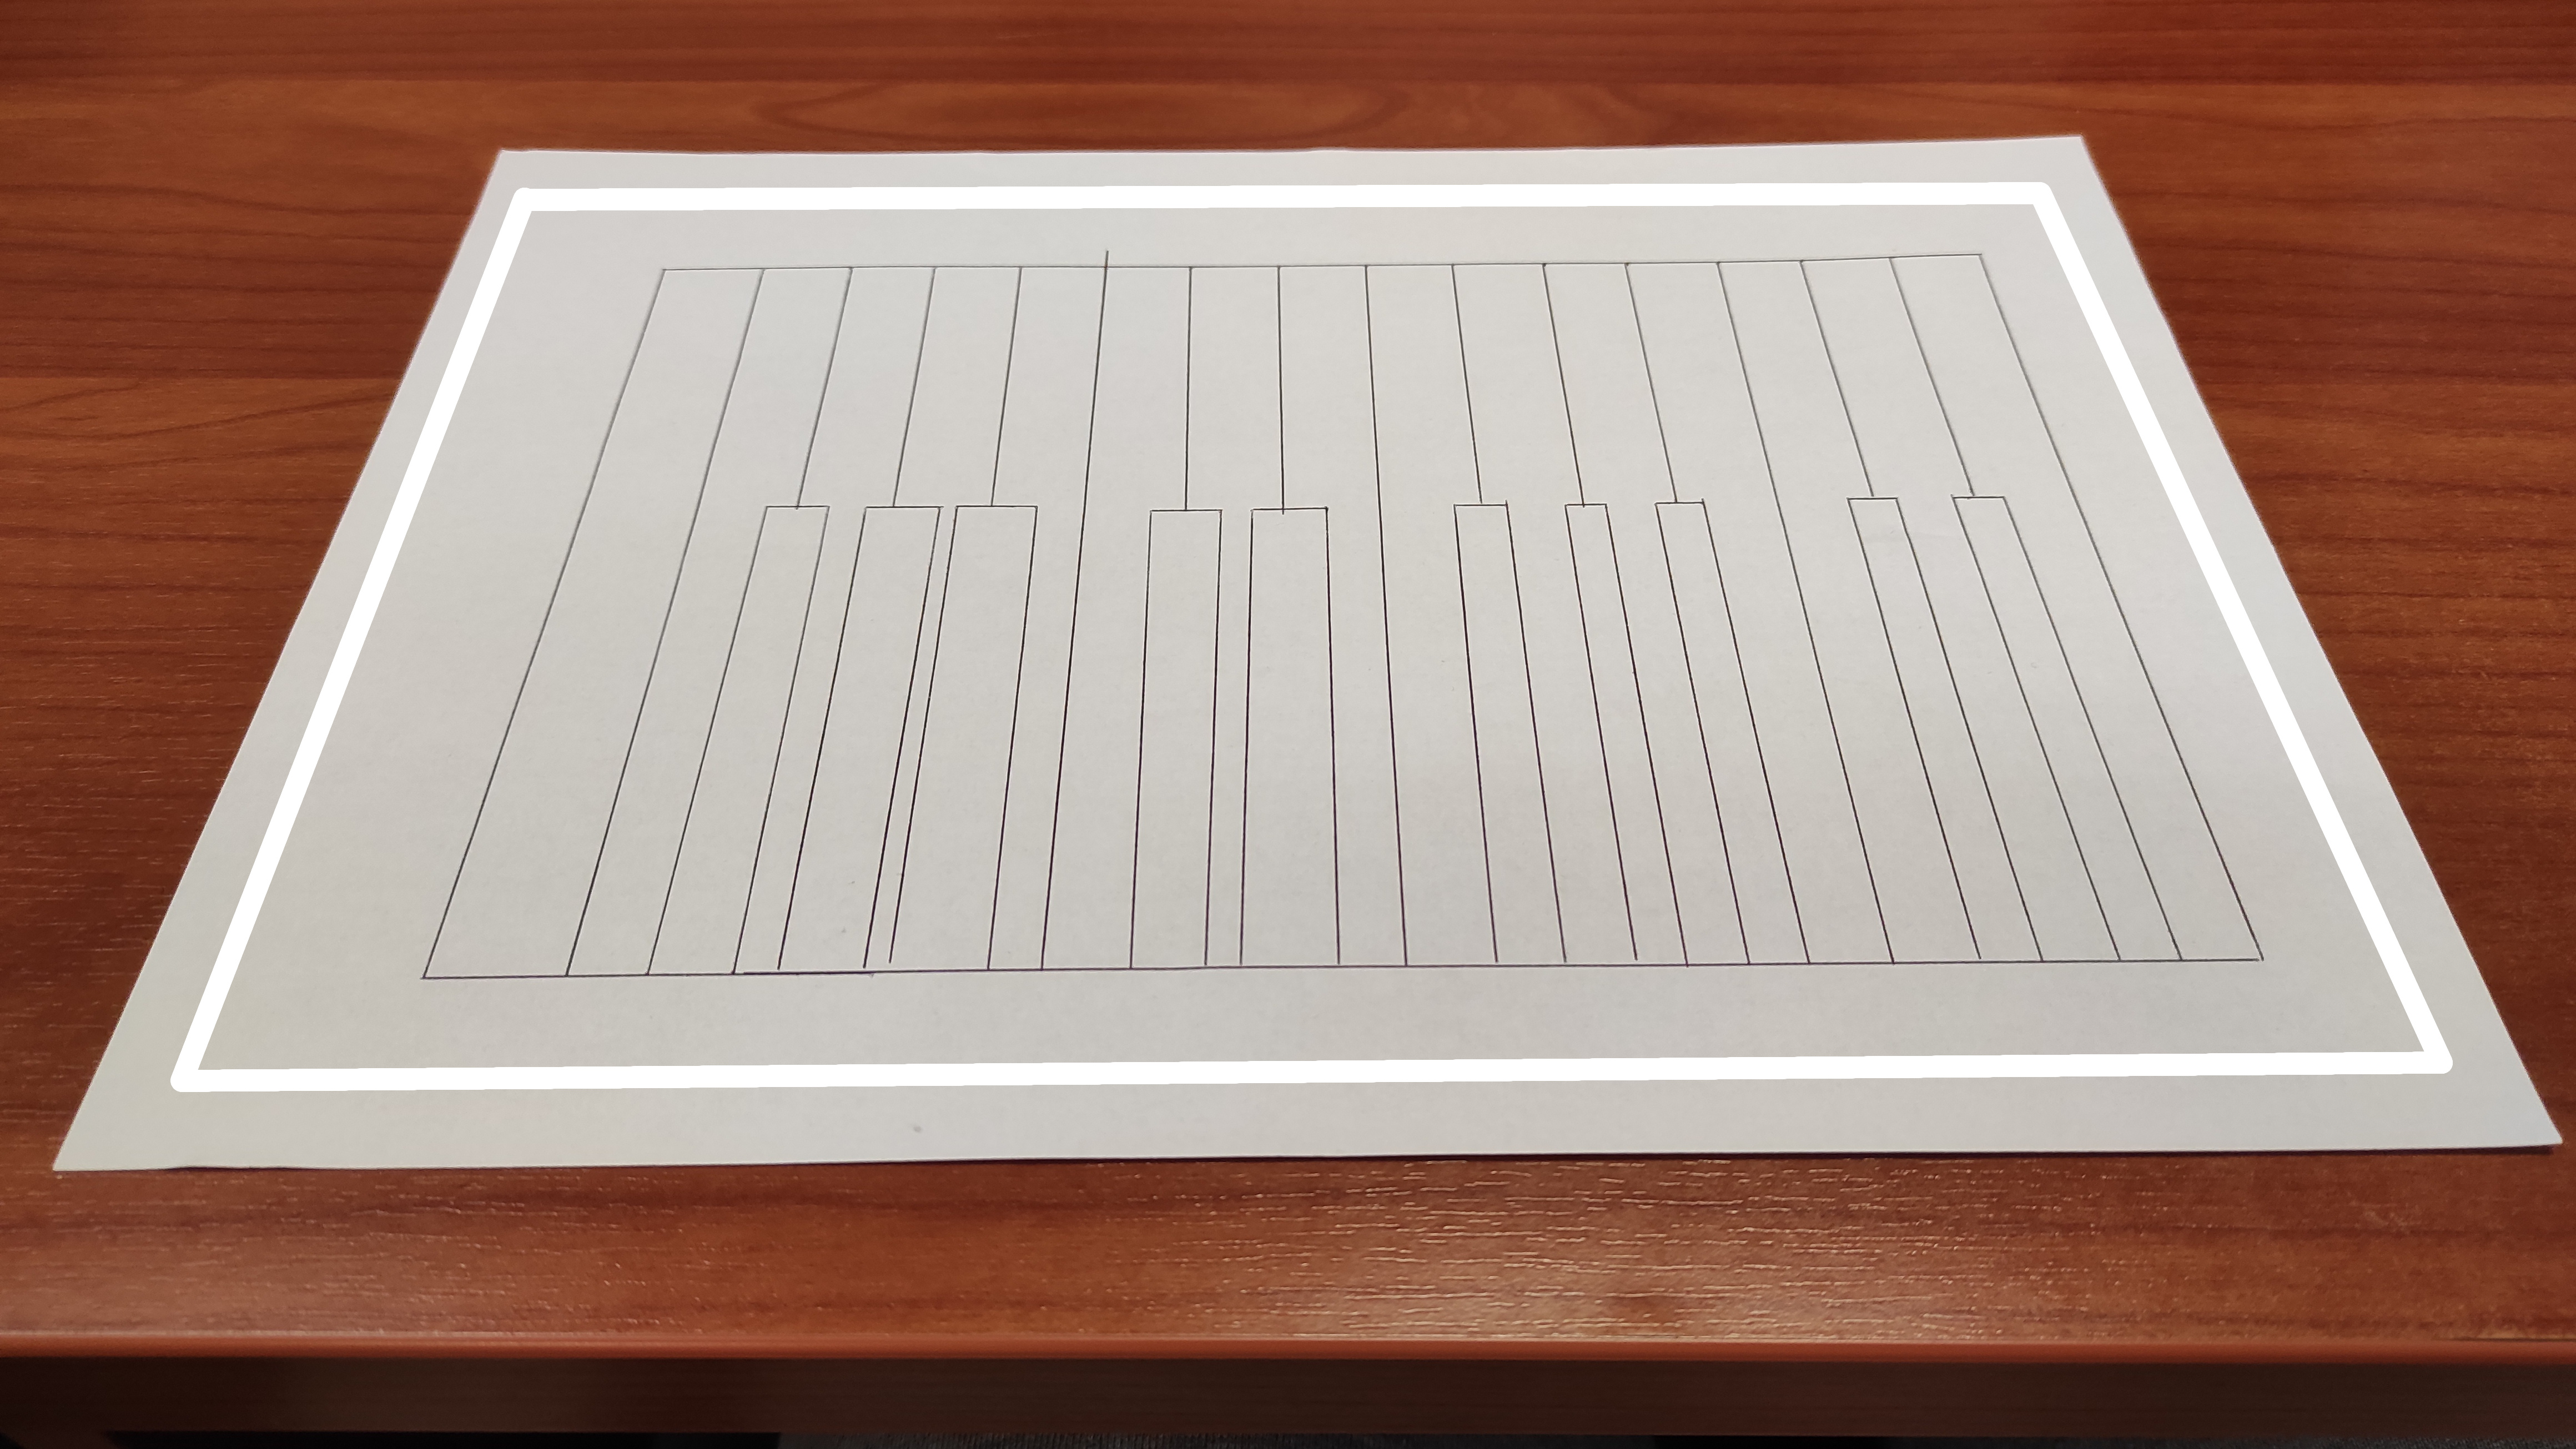
\includegraphics[width=\textwidth]{images/application/45deg/camera-with-frame}
		\caption{}
		\label{fig:perimeter}
	\end{subfigure}
	\hfill
	\begin{subfigure}{0.49\textwidth}
		\centering
		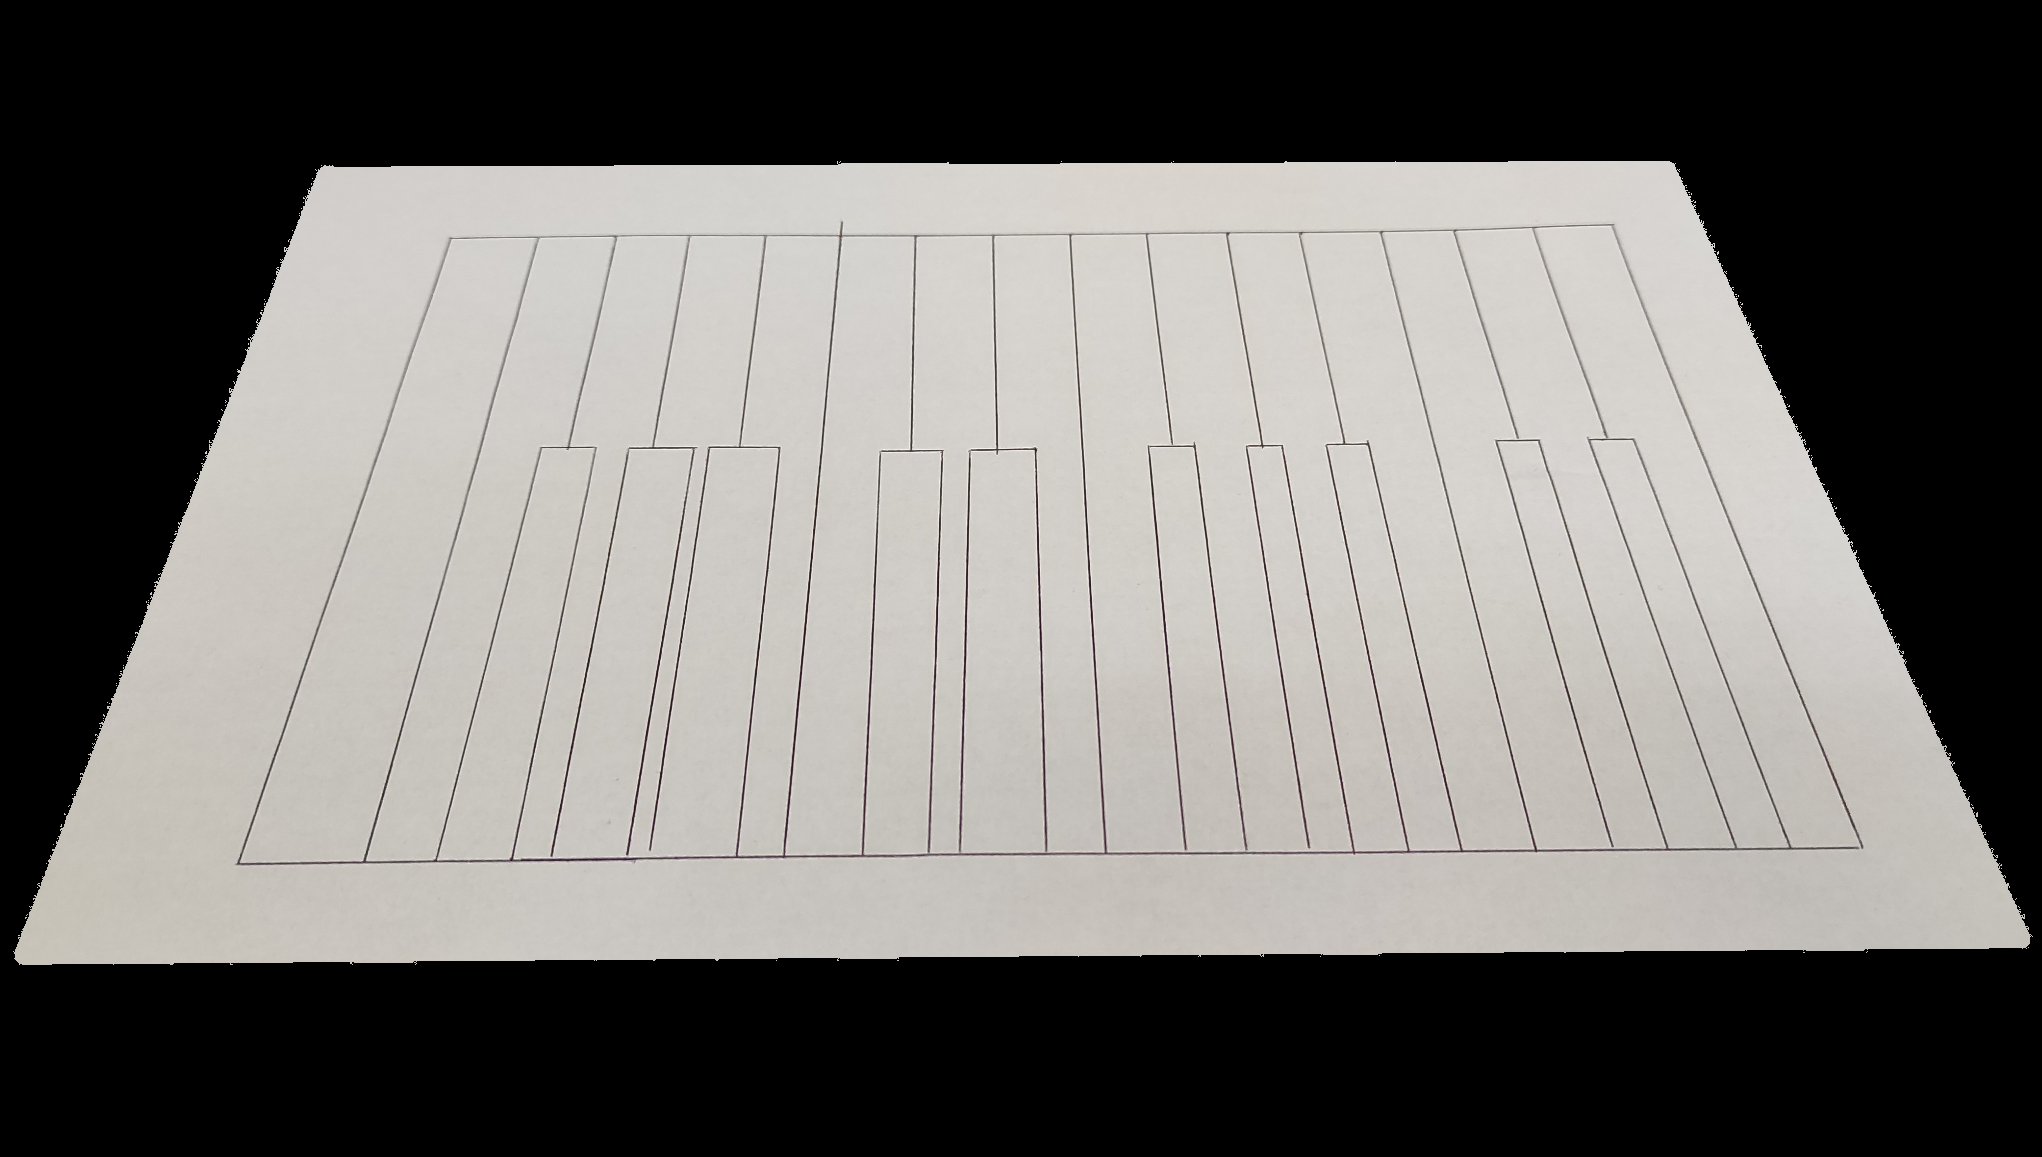
\includegraphics[width=\textwidth]{images/application/45deg/masked}
		\caption{}
		\label{fig:mat}
	\end{subfigure}
	\hfill
	\begin{subfigure}{0.49\textwidth}
		\centering
		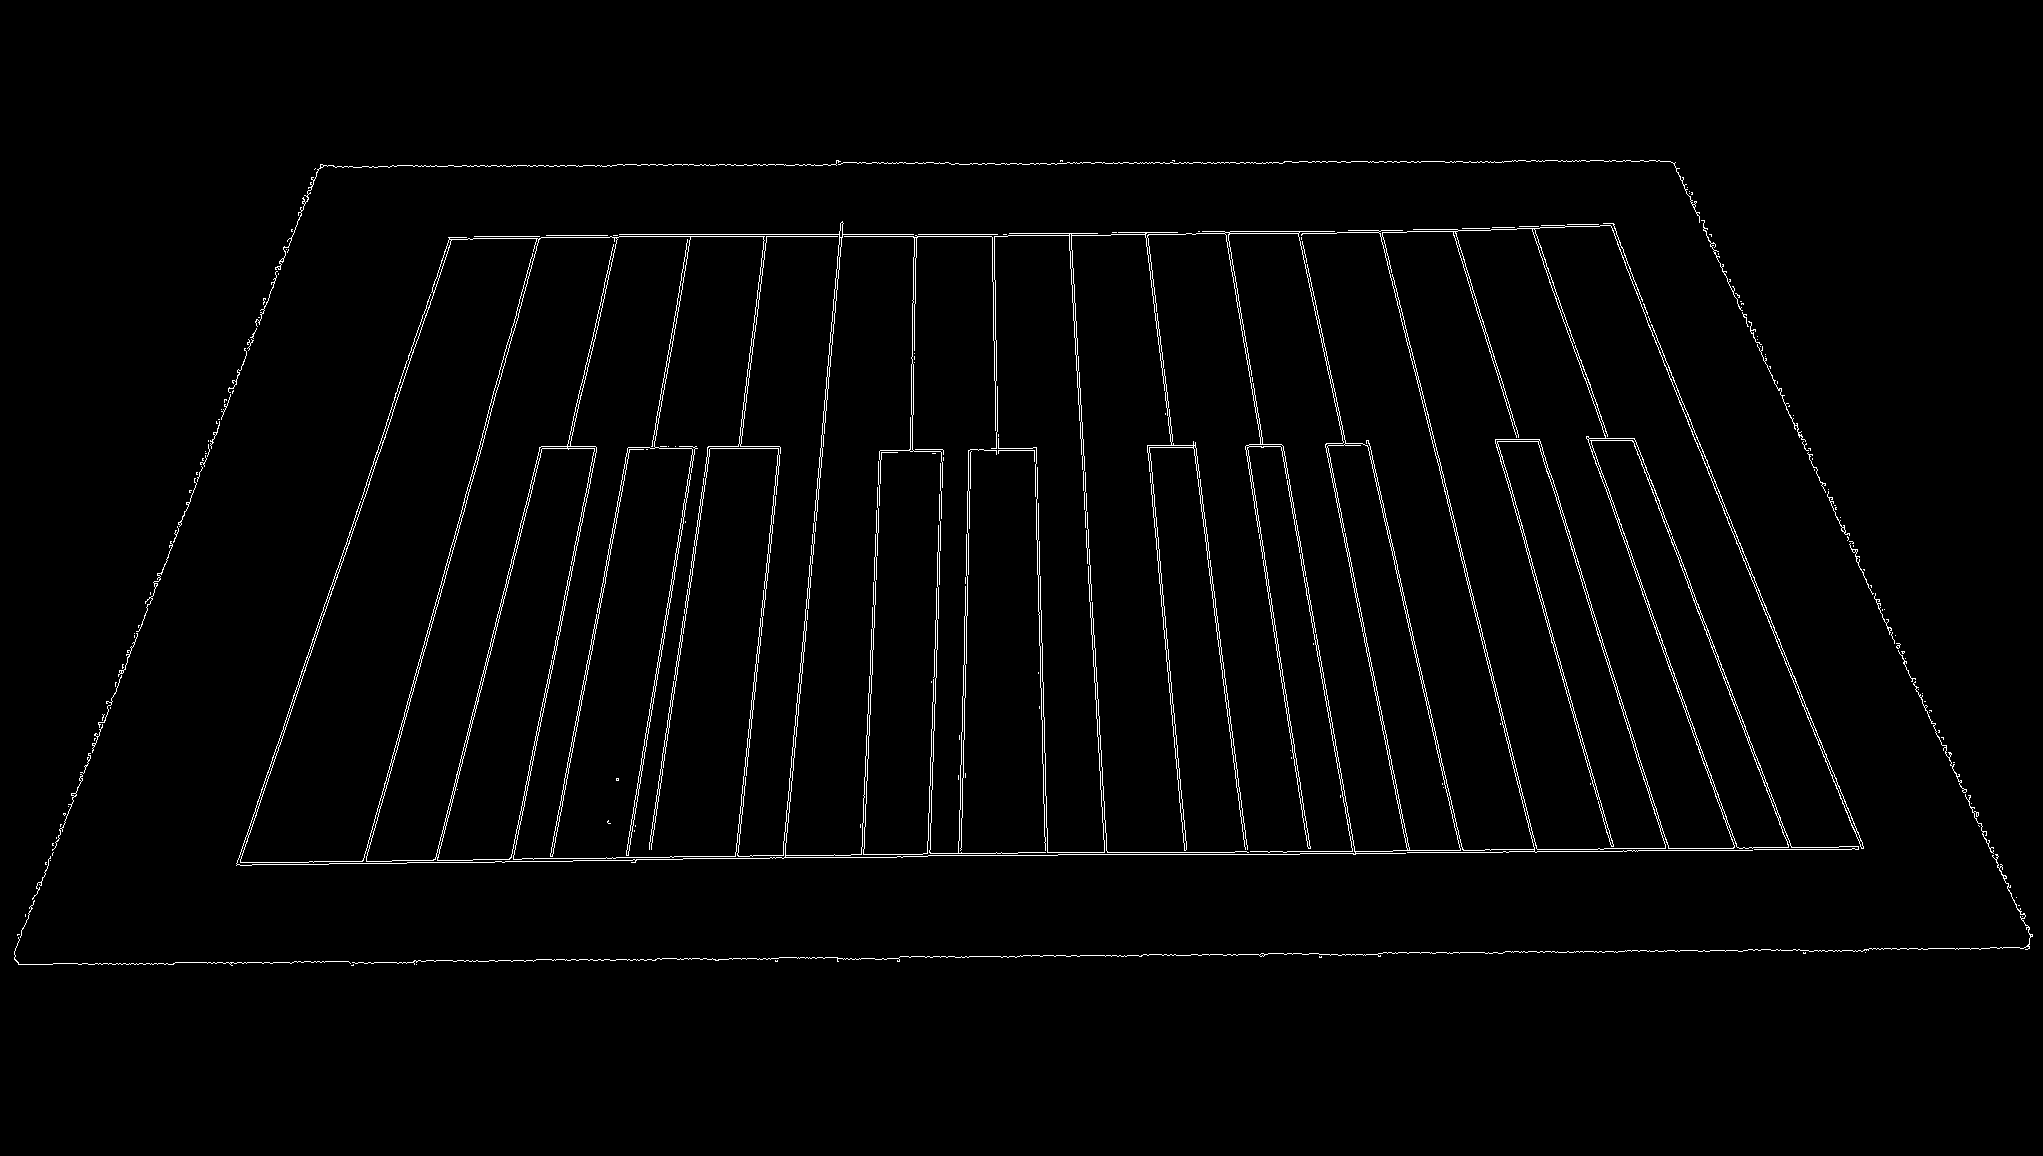
\includegraphics[width=\textwidth]{images/application/45deg/canny}
		\caption{}
		\label{fig:canny}
	\end{subfigure}
	\hfill
	\begin{subfigure}{0.49\textwidth}
		\centering
		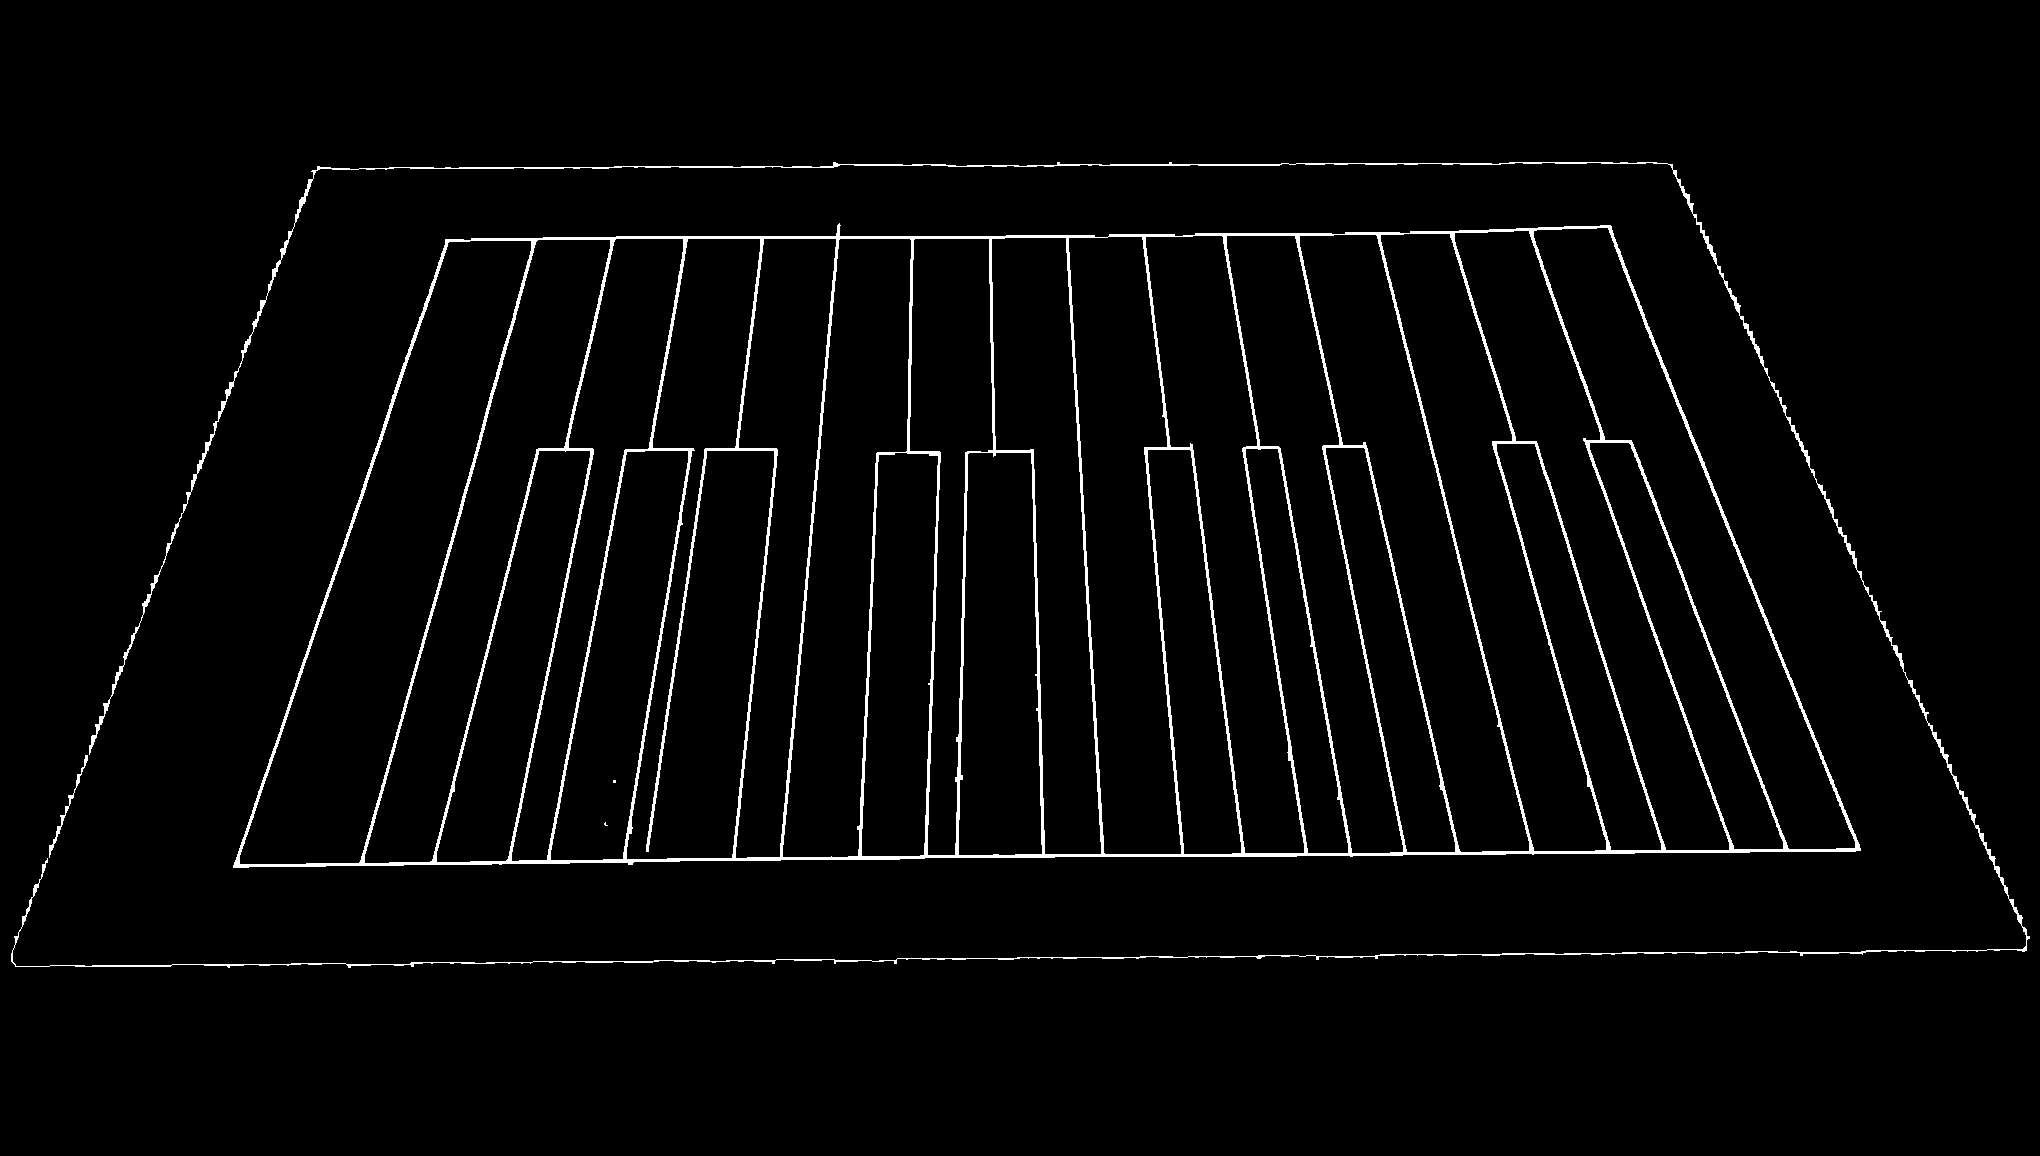
\includegraphics[width=\textwidth]{images/application/45deg/canny-closed}
		\caption{}
		\label{fig:canny-closed}
	\end{subfigure}
	\hfill
	\begin{subfigure}{0.49\textwidth}
		\centering
		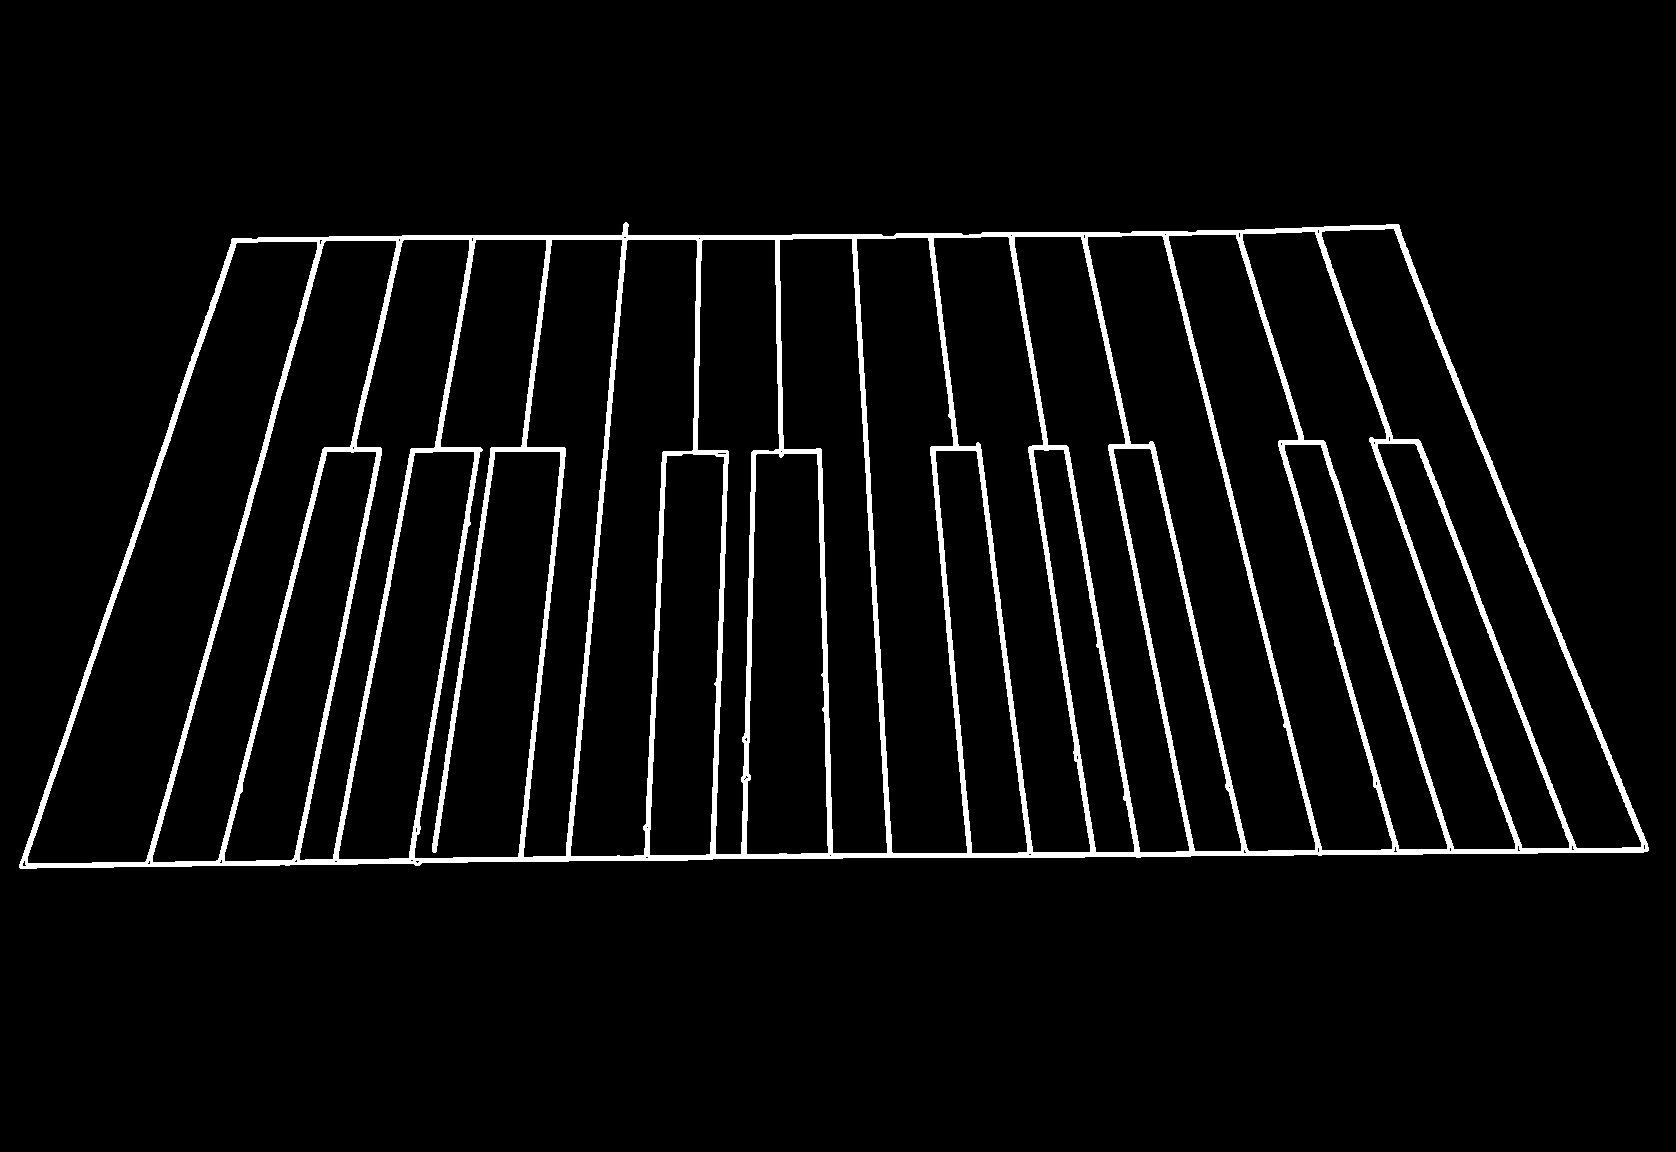
\includegraphics[width=\textwidth]{images/application/45deg/contours}
		\caption{}
		\label{fig:contours}
	\end{subfigure}
	\hfill
	\begin{subfigure}{0.49\textwidth}
		\centering
		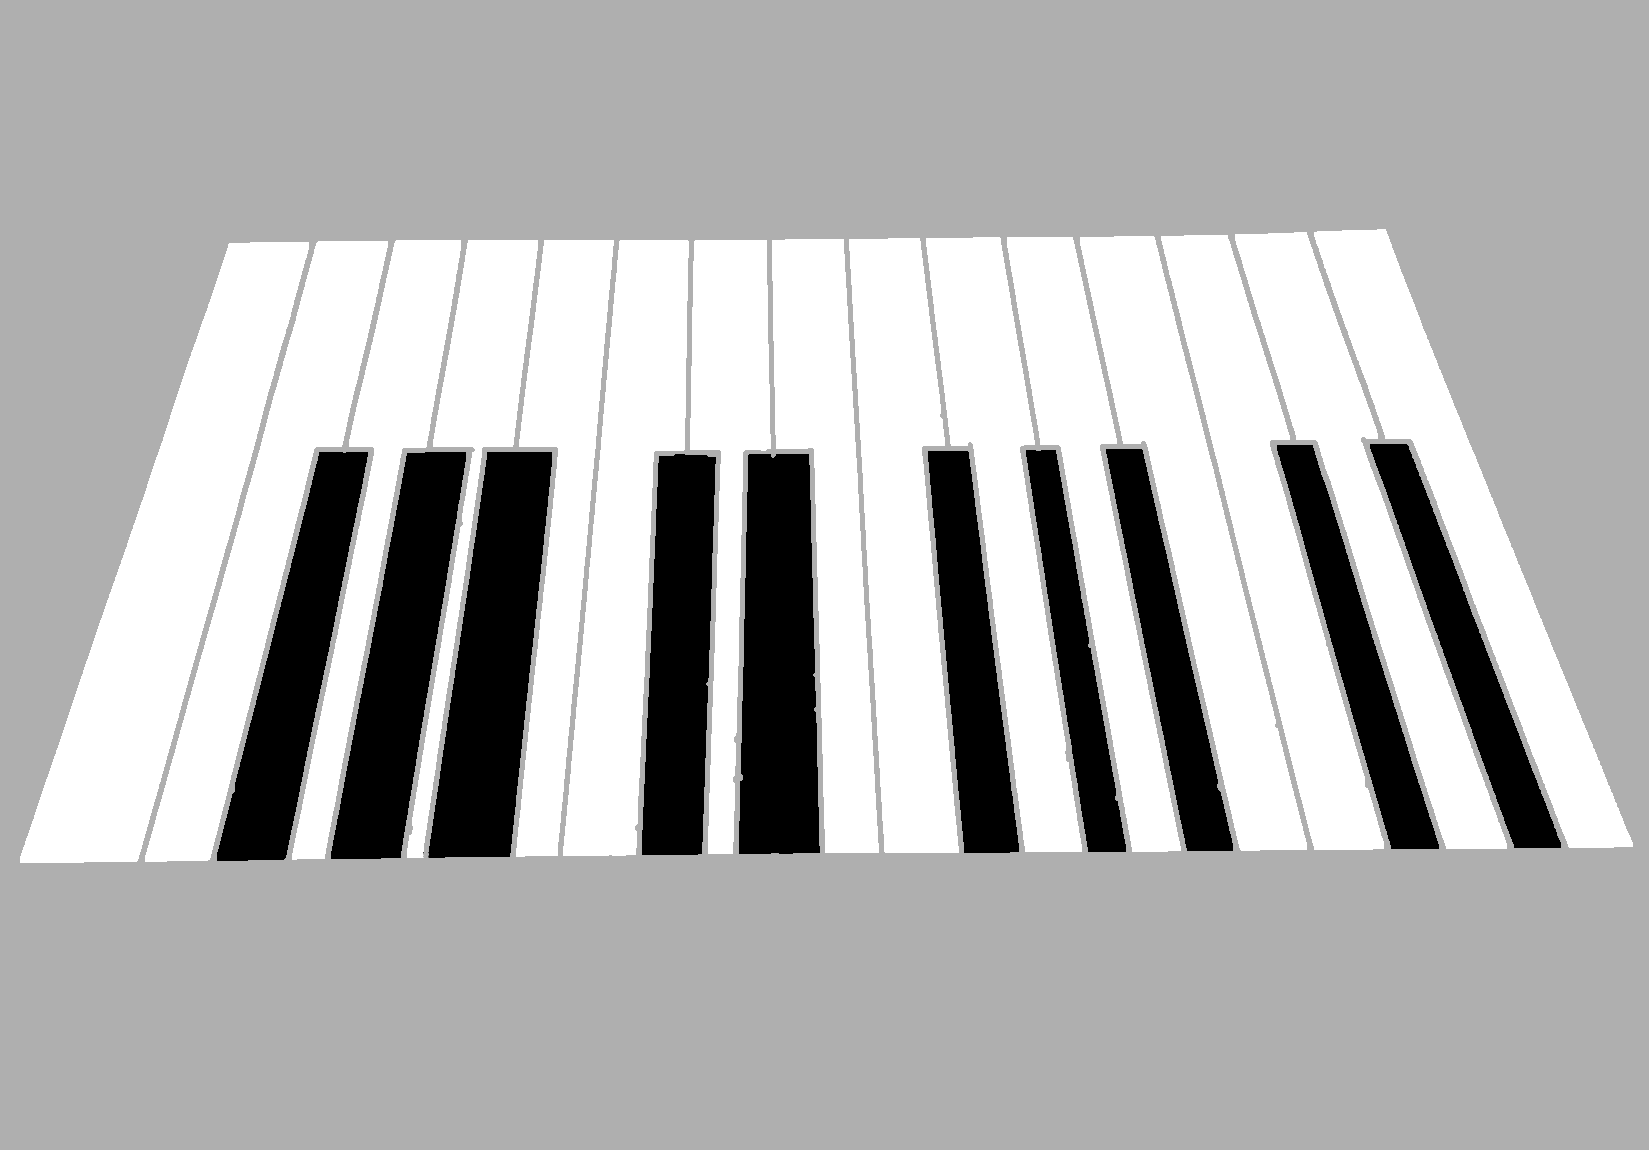
\includegraphics[width=\textwidth]{images/application/45deg/tiles-overlay}
		\caption{}
		\label{fig:tiles-overlay}
	\end{subfigure}
	\hfill
	\begin{subfigure}{0.49\textwidth}
		\centering
		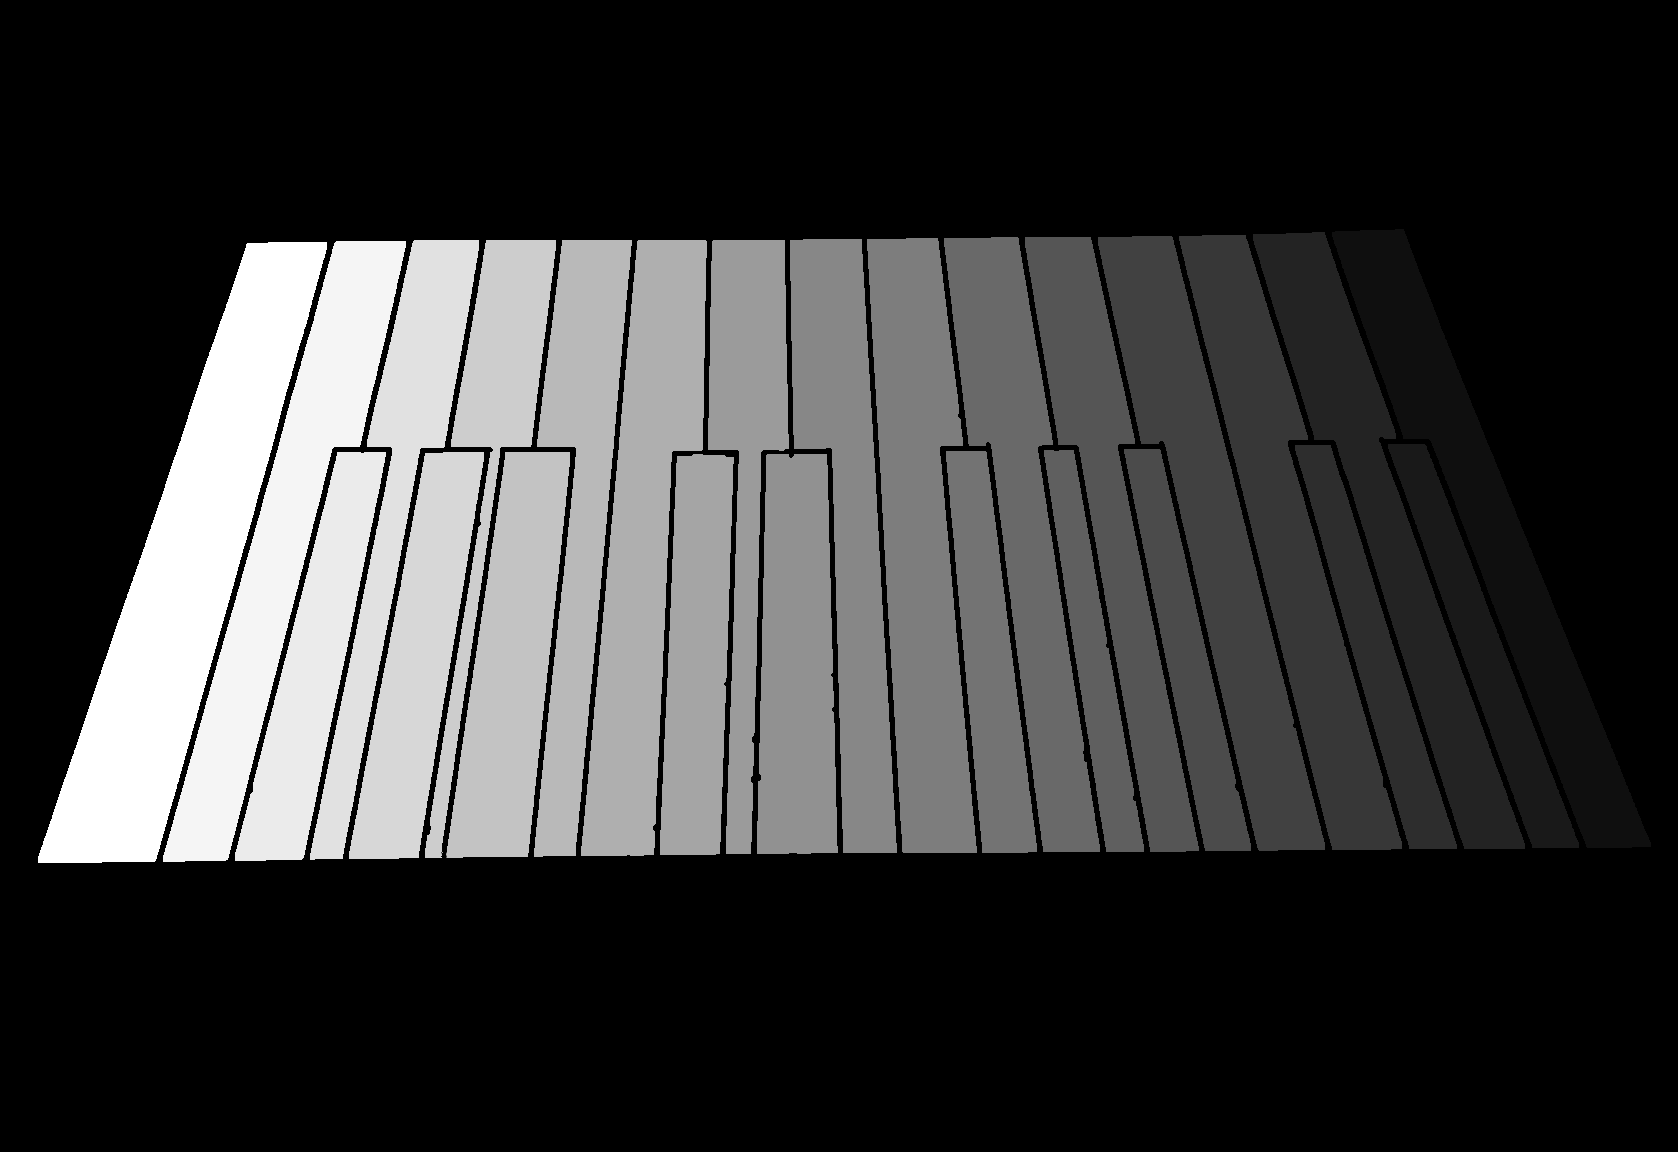
\includegraphics[width=\textwidth]{images/application/45deg/notes-overlay}
		\caption{}
		\label{fig:notes}
	\end{subfigure}
	\caption{
		Keyboard detection pipeline.
		(a) Perimeter;
		(b) Keyboard after background subtraction;
		(c) Canny edge;
		(d) Canny edge after morphological closure;
		(e) Contour detection (after filter);
		(f) Tiles overlay (not in transparency for visibility);
		(g) Notes indexes (brightness enhanced for visibility).
	}
	\label{fig:preprocessing}
\end{figure}

\subsubsection{Keyboard presets}
In this mode, instead of using a photo taken by the user to search for the keyboard and show the keys thus detected,
the shape and position of the keys that the application expects to use is shown directly.

The user can download and print out on an A4 sheet the model of the keyboard that the
application shows on the screen and must position it at the guides shown on the interface.
In this way, the user's physical keyboard will perfectly match the one presented by the application,
ensuring optimal performance and realism.

The PDF files for printing the keyboard presets will be available for download on the project's website.
The different keyboard models made available by default by the application are shown in \autoref{fig:presets}.

\begin{figure}[ht]
	\centering
	\begin{subfigure}{0.49\textwidth}
		\centering
		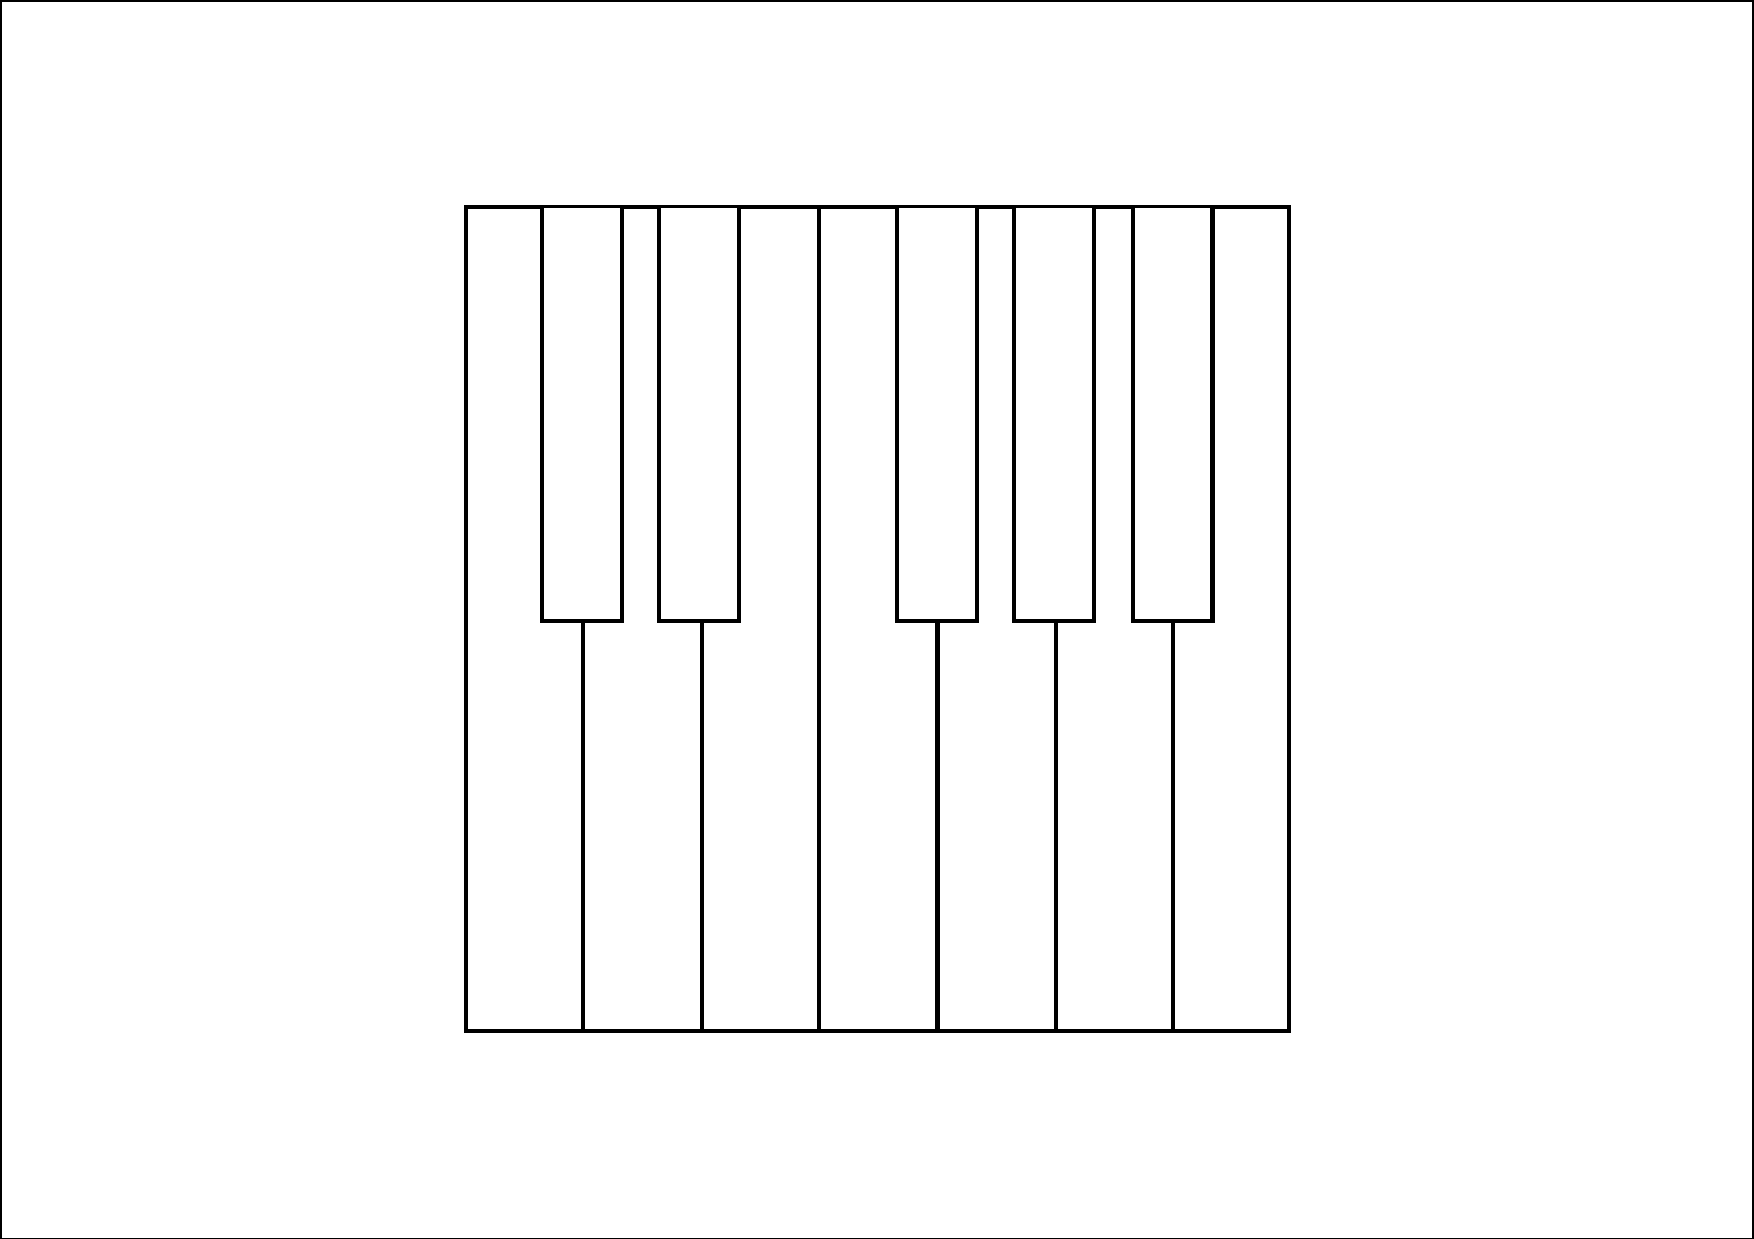
\includegraphics[width=\textwidth]{application/presets/keyboard-preset-1}
		\caption{}
		\label{fig:preset-1}
	\end{subfigure}
	\hfill
	\begin{subfigure}{0.49\textwidth}
		\centering
		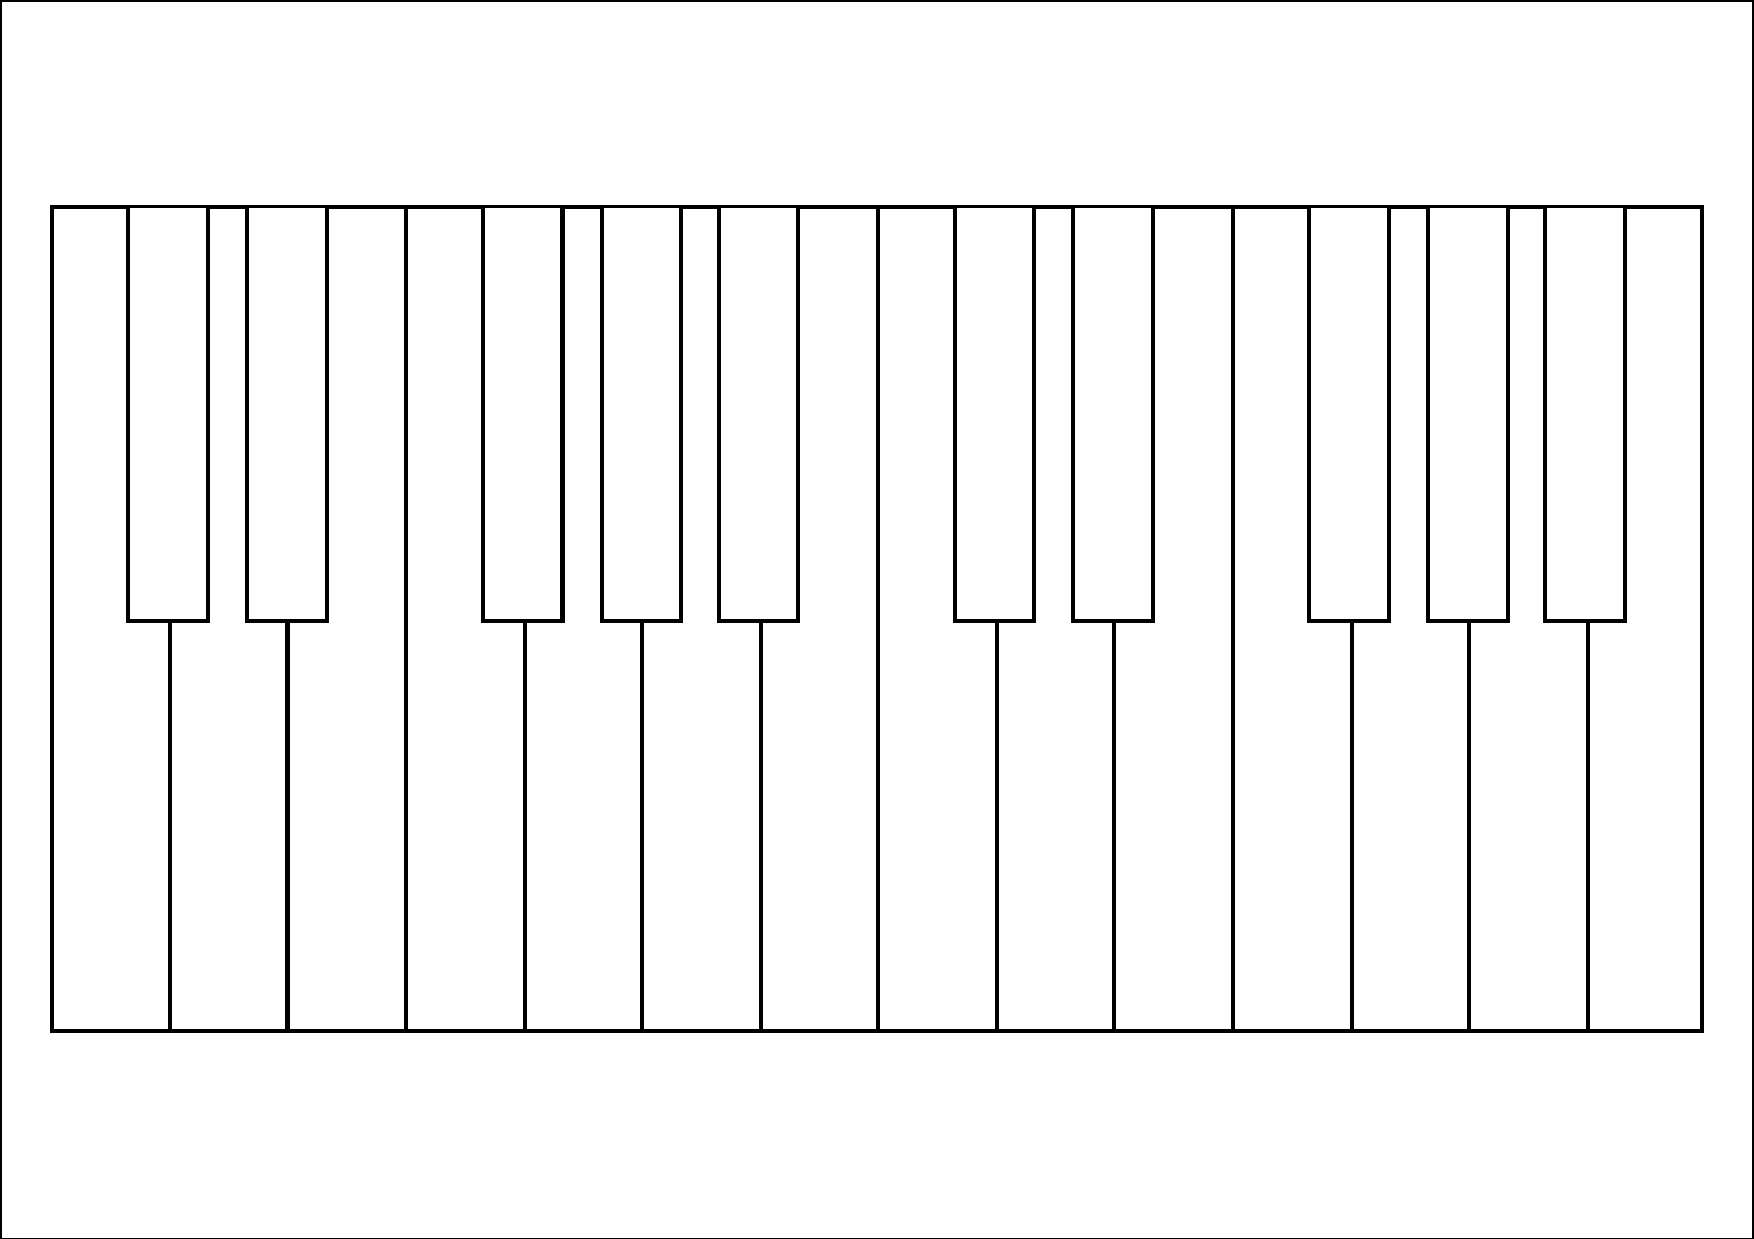
\includegraphics[width=\textwidth]{application/presets/keyboard-preset-2}
		\caption{}
		\label{fig:preset-2}
	\end{subfigure}
	\caption{
		Keyboard presets different keyboard sizes.
		(a) One octave keyboard;
		(b) Two octaves keyboard.
	}
	\label{fig:presets}
\end{figure}
